\documentclass{article}

\usepackage[english]{babel}
\usepackage[letterpaper,top=2cm,bottom=2cm,left=3cm,right=3cm,marginparwidth=1.75cm]{geometry}
\usepackage{amsmath}
\usepackage{graphicx}
\usepackage{float}
\usepackage{subcaption}
\usepackage[colorlinks=true, allcolors=blue]{hyperref}

\title{Determining the accuracy of FreeRunning mode versus Parallel mode as well as the accuracy of Equi-Width Histograms versus Equi-Depth Histograms using SPCSimLib \cite{SPCSimLib}}
\author{NotSureHowManyPeopleIShouldPutHere \& Elliott H. VanOrman}

\begin{document}
\maketitle

\begin{abstract}
This paper compares the error in results of a Single Photon Camera (SPC) in parallel mode versus freerunning mode, as well as comparing error when using Equi-Width Histograms (EWH) and Equi-Depth Histograms (EDH).
Data was collected using the python library SPCSimLib, specifically by simulating a single SPC pixel, and measuring the error each method produced.
Our analysis showed that when FreeRunning mode was used, the resulting measurements matched with reality more than when parallel mode was used, to a statistically significant level.
from this, we concluded that FreeRunning mode produced more accurate results than parallel mode,
\end{abstract}

\section{Introduction}

Single Photon Cameras, or 'SPC's for short, are cameras that function similarly to LIDAR, in that they produce 3D photographs by measuring the time it takes for light to travel to a point and bounce back. unlike LIDAR however, SPCs use individual photons instead of lasers.

when a picture is taken, the SPC begins sending out pulses of photons towards the thing it is taking a picture of. when these photons are reflected back onto the detector, it records the timestamp. There are almost always ambient photon levels, however, meaning that while timestamps do cluster around the 'true' time it took photons to reflect back, there are a certain number of 'noise' timestamps due to background illumination. there are multiple methods to determine when the true center of the pulse, called the 'peak' is located. after the 'peak' is located, it is used to determine the distance from the camera of the pixel using the formula \[\frac{T*\frac{1}{2}}{C}\] where $T$ is the time it took for photons to reflect back to the detector and $C$ is the speed of light.

the exact steps of sorting out noise from true varies based on method: When using Equi-Width histograms, a histogram is constructed with buckets of equal width but variable depth. The center of the bucket with the most detections is recorded as the 'peak' of the pulse. When using Equi-Depth histograms, a histogram is constructed with buckets of variable width but equal depth. The center of the bucket with the thinnest width is recorded as the 'peak' of the pulse.

Due to the physical limitations of SPC cameras, however, photon readings over time do not always match reality. when a detector is hit by a photon, it takes a certain amount of time for said detector to log a timestamp. While this time is in progress, the detector cannot record new hits. in other words, a detector cannot start recording a new timestamp until it has finished recording the first, meaning photons that hit the detector during that recording time go undetected. this time is refered to as 'deadtime'

how SPC cameras deal with deadtime also varies based method, or, in this case, Mode. in Parallel mode, detectors are reset at the begining of each cycle, regardless of whether or not they've detected anything. this method leads to photon readings to be skewed to the right. This is due to early photons triggering deadtime, preventing pixels from detecting photons until late into a detection-cycle.  In asynchronous mode, also called freeRun mode, detectors do not reset at the beginning of each cycle, leading to relatively less skewed data.

Additionally, the length the laser will fire (refered to as FWHM, or Full Width at Half Maximum, refering to the length of the curve of intensity of the laser when it fires), also varies, and said length could also affect the error of the laser, though how precisely was somewhat uncertain.

As I have explained, there are many methods that can be used to receive and interpret data from SPCs, but it has not yet been determined which produces the most accurate results. It was hypothesized that Equi-depth histograms would produce more accurate results than Equi-Width histograms, that asynchronous (non-freerunning) mode would produce more accurate results than parallel (freerunning) mode, and that 1.5 FWHM would produce the same amount of error as 5.0 FWHM.



\section{Method}
In order to determine what produced the most accurate results, we used the Python library SPCSimLib \cite{SPCSimLib} to simulate a pixel of an SPC. Within each pixel, we simulated taking a picture with an SPC. then, we subtracted the 'true distance' (the distance from the camera the surface being photographed was in the simulation) from the 'estimated distance' (the distance from the camera of the same surface that the SPC in the simulation estimated). after taking this difference, we normalize it by dividing it by the scale of the distance. This normalized difference is what we are referring to when we say 'error'. In order to produce the most accurate results, we ran 10 tests for every level of attenuation, then took the average in order to minimize the effects of fluctuations. 

After taking this error, we recorded it in a series of publicly available data sets \href{https://github.com/yggaraxyg/SPCErrorLowerer/tree/master/RunData}{here}. Once we had this data recorded, we proceeded to graph it in the formats shown below, publically avalable \href{https://github.com/yggaraxyg/SPCErrorLowerer/tree/master/Graphs}{here}.

\begin{figure}[H]
\centering
\begin{subfigure}[b]{1\textwidth}
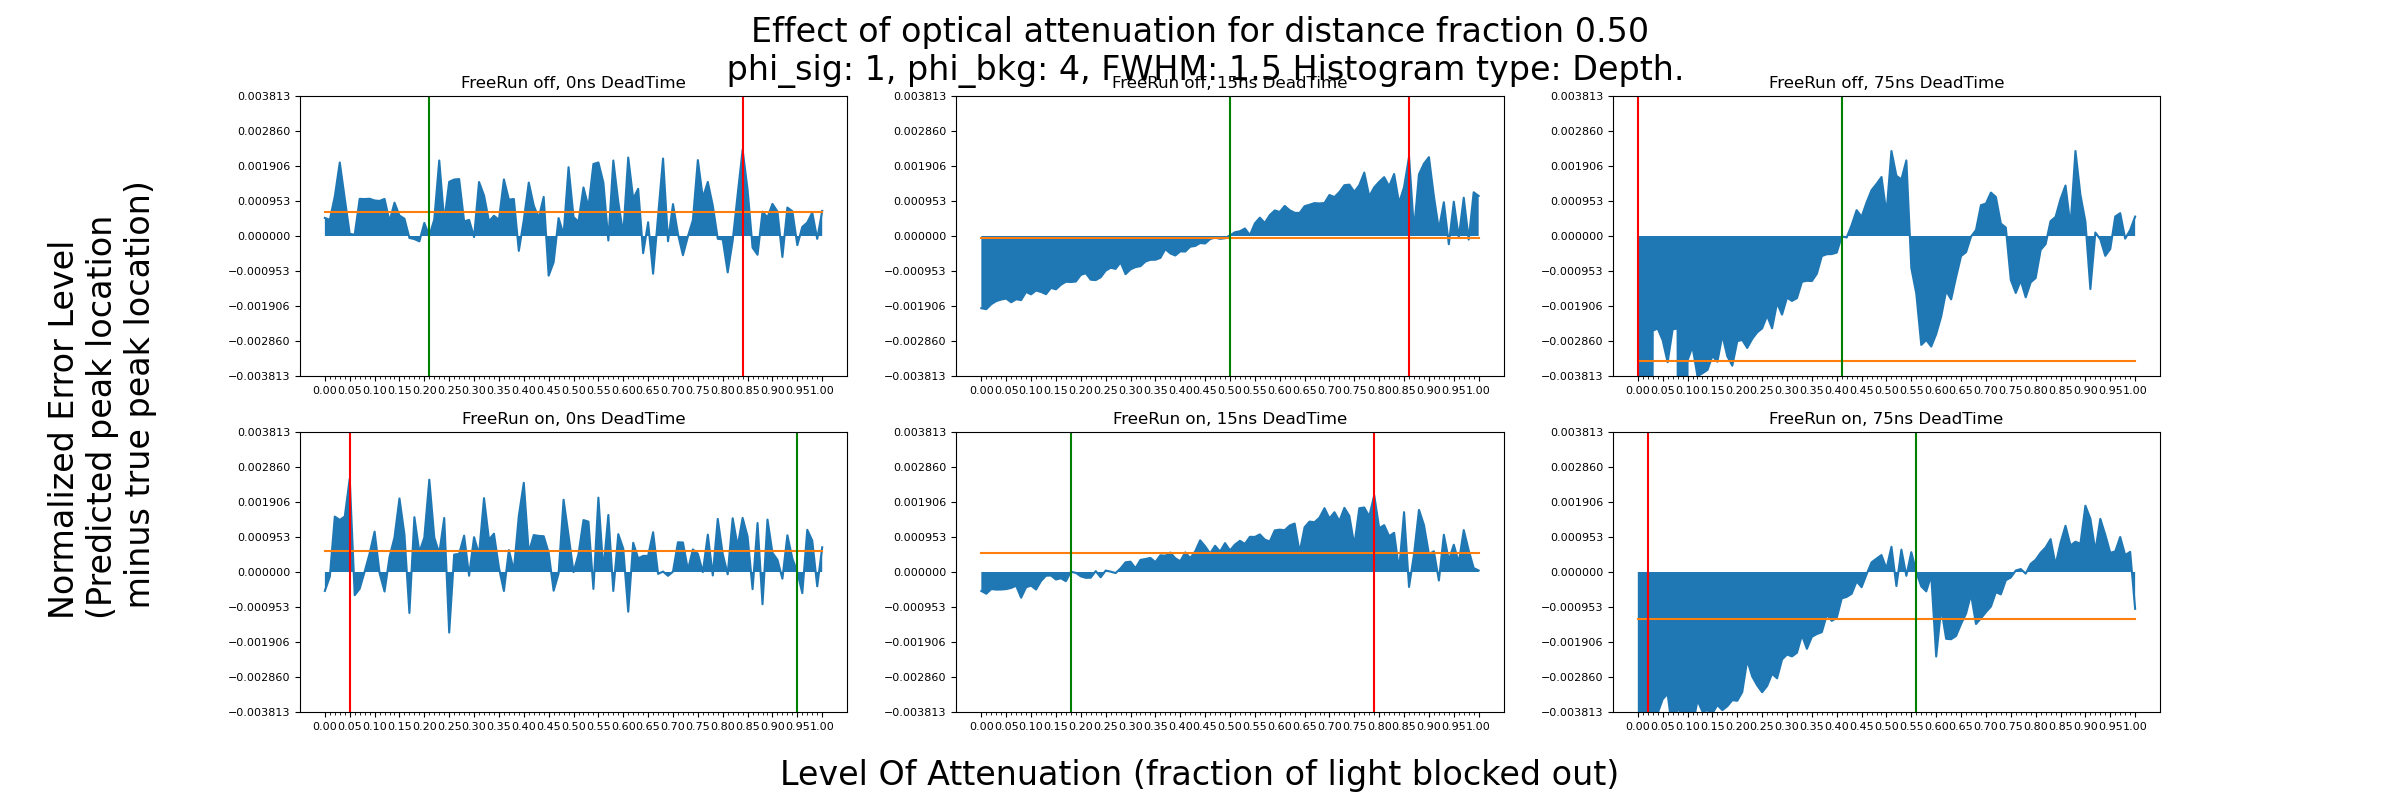
\includegraphics[width=1\linewidth]{SharedyExample.png}
\label{fig:Ng1}
\end{subfigure}
\begin{subfigure}[b]{1\textwidth}
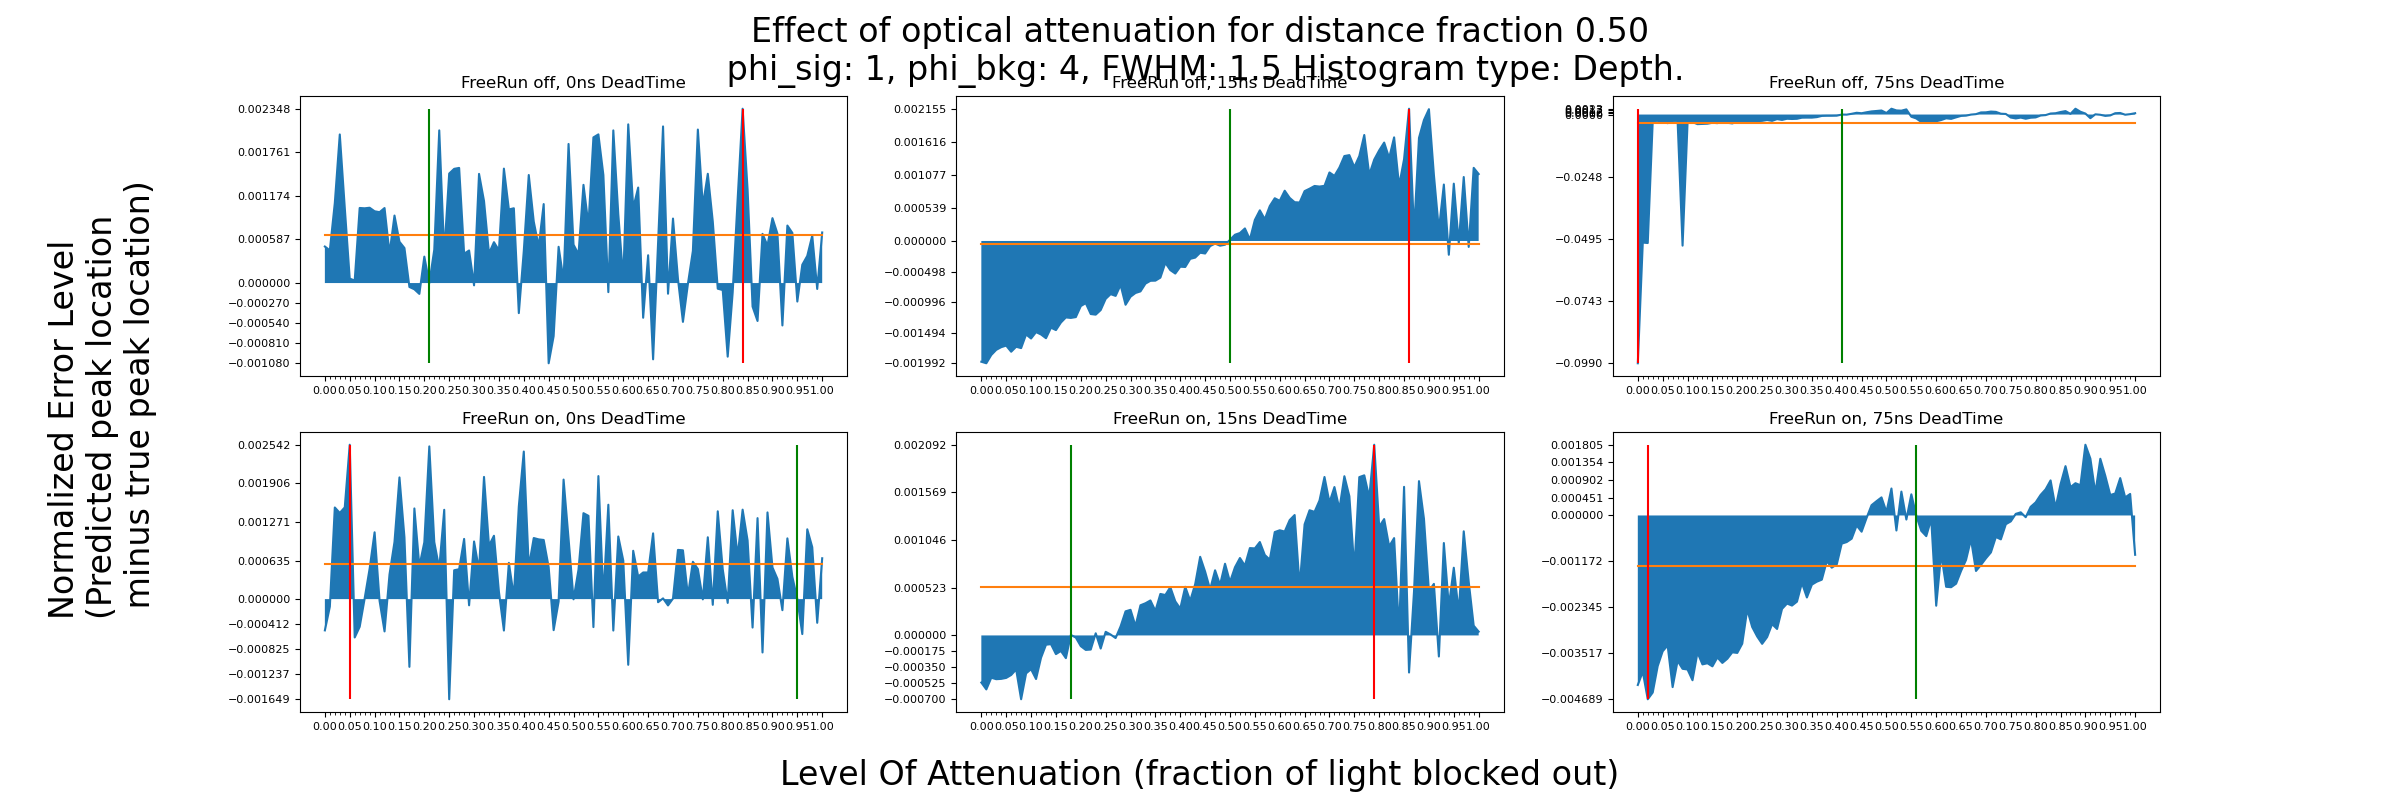
\includegraphics[width=1\linewidth]{ZoomedyExample.png}
\label{fig:Ng2}
\end{subfigure}

\caption{\label{fig:Data}The top graph and the bottom graph present the same data in two different formats. the top graph represents error on the same scale across all graphs, while the bottom represents each dataset with it's own scale. Blue represents normalized error. Orange is the mean error for all attenuation values. Red is the attenuation value which produced the least accurate result. Green is the attenuation value which produced the most accurate result.}
\end{figure}

in addition, we ran Paired-T tests on the data to check our hypotheses. to do this, we put all our data in two large datasets for every 


\section{Results}
Following the creation of the graphs and the statistical tests, we are able to make the following statements with 99.99999\% certainty: (all P-values were less than 0.0000001)

\begin{itemize}
  \item EDH Error Calculation produces more error than EWH Error Calculation
  \item FreeRun simulations produces less error than Non-Freerun simulations
  \item 1.5 FWHM simulations produces less error than 5.0 FWHM simulations
\end{itemize}

Graphs showing examples of said trends are below:

\begin{figure}[H]
\centering
\begin{subfigure}[b]{1\textwidth}
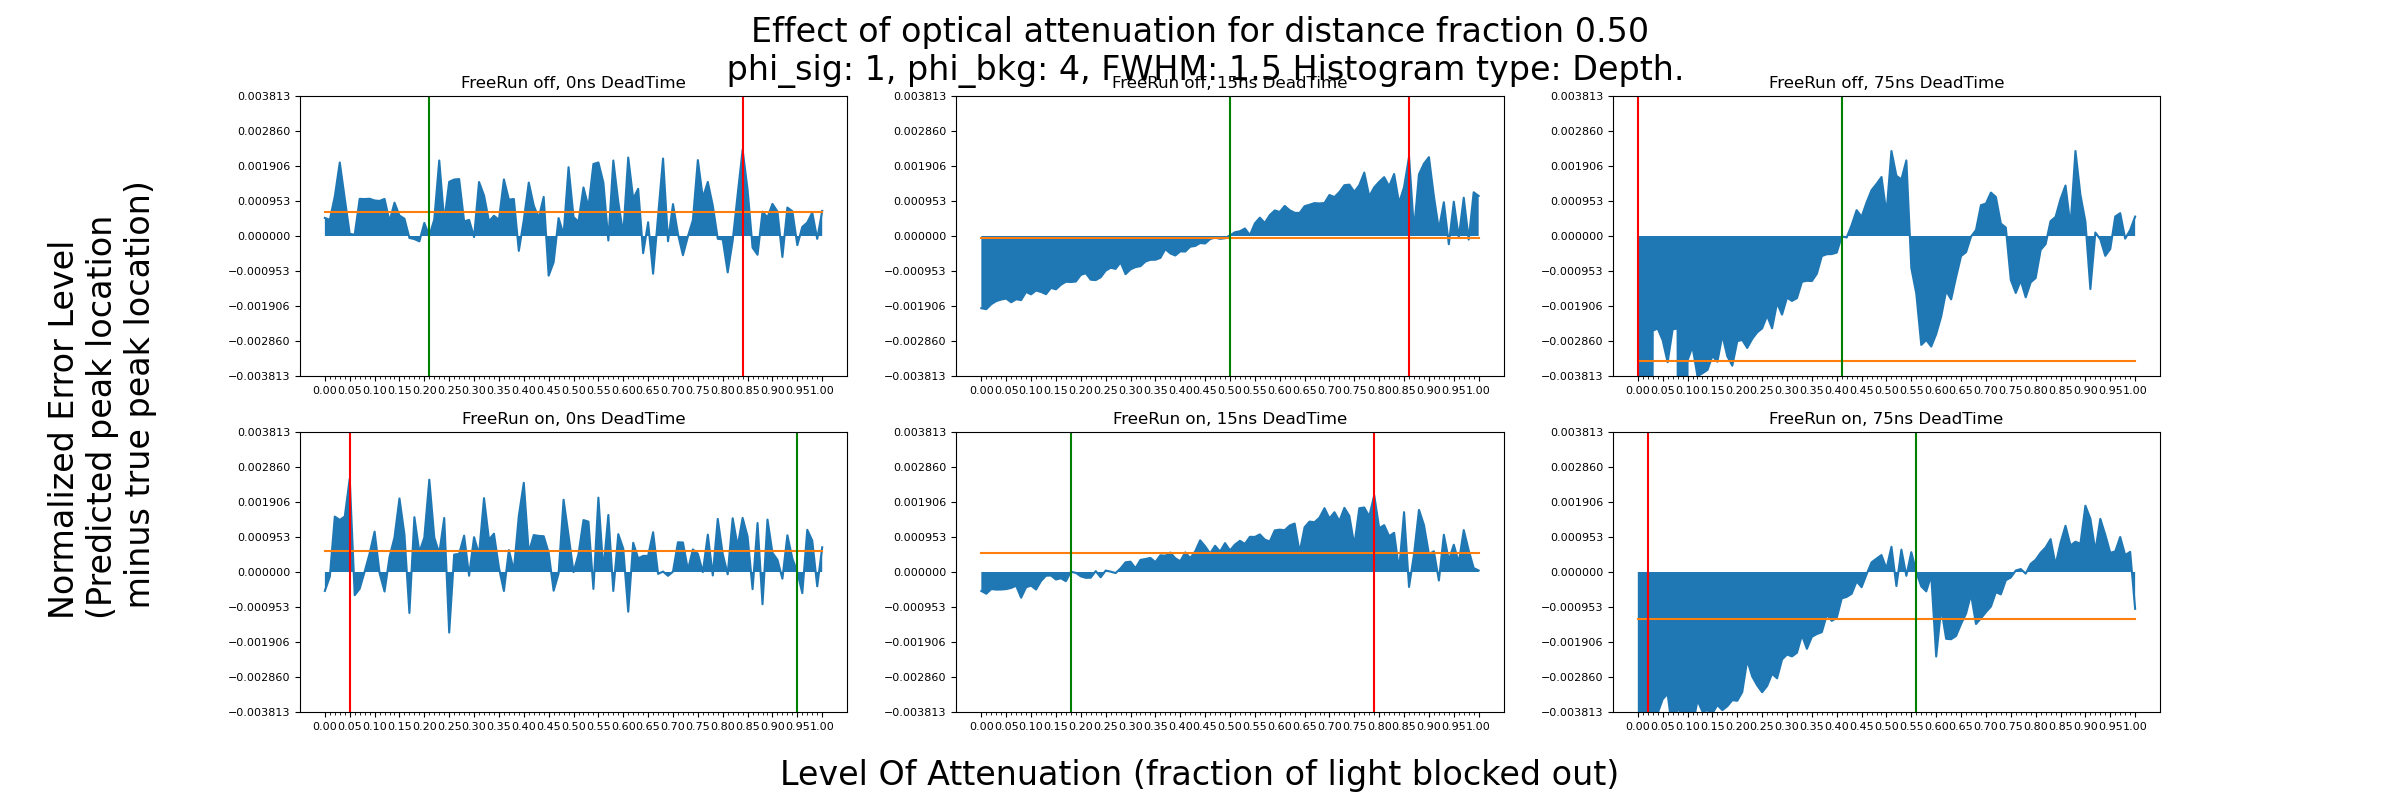
\includegraphics[width=1\linewidth]{SharedyExample.png}
\label{fig:Ng1}
\end{subfigure}
\begin{subfigure}[b]{1\textwidth}
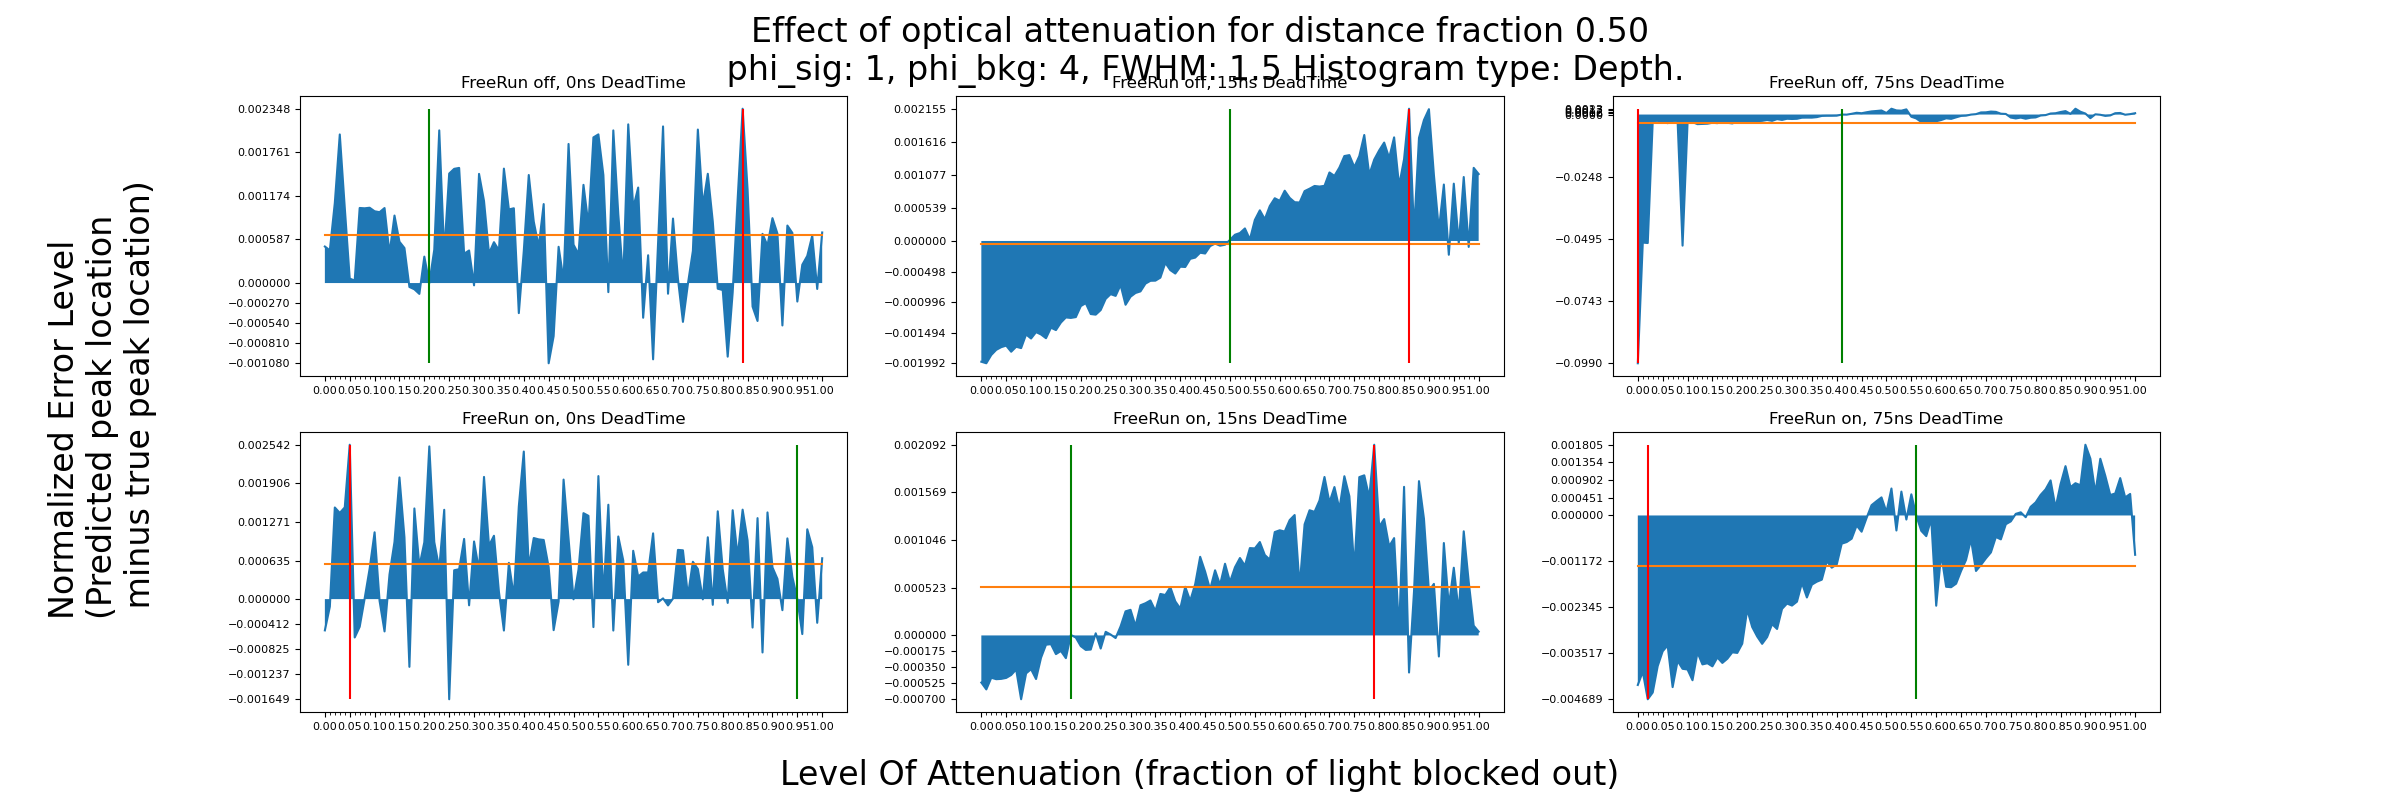
\includegraphics[width=1\linewidth]{ZoomedyExample.png}
\label{fig:Ng2}
\end{subfigure}
\caption{\label{fig:Data}EDH vs EWH}
\end{figure}

\section{Discussion}

\section{Conclusion}

\bibliographystyle{alpha}
\bibliography{sample}
\end{document}
